\subsection{URL dispatching}
\label{url_dispatching}

Orice aplicatie care distribuie informatia sub forma unor pagini web are un sistem de traducere a solicitarilor clientilor (URL) catre elemente executabile din interior. 

In cazul framework-ului Spring, schema folosita pentru URL-dispatching este descrisa mai jos :

\bigskip

\begin{center}
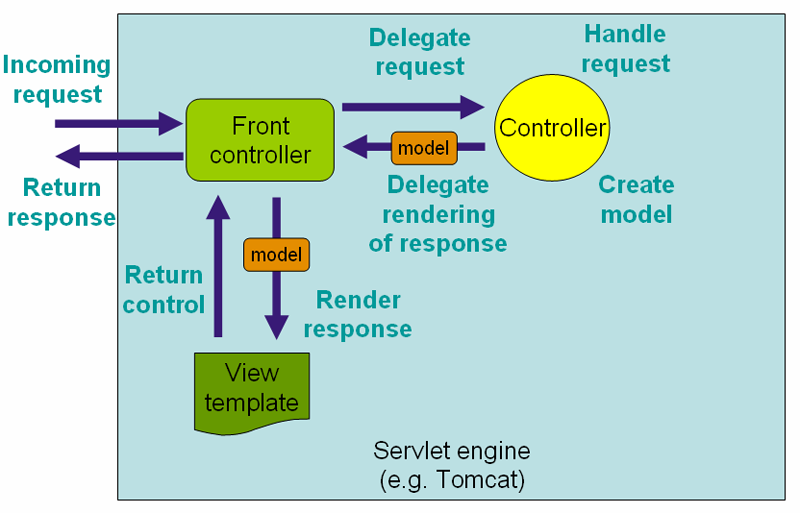
\includegraphics[width=\textwidth]{mvc.png}
\end{center}

\bigskip

Se utilizeaza un design-pattern de tip "Front Controller", rol jucat de catre "DispatcherServlet" \footnote{\url{http://docs.spring.io/spring/docs/3.2.x/spring-framework-reference/html/mvc.html}}.
DispatcherServlet este chiar un servlet si este declarat ca atare in fisierul de configurare "web.xml"; se mapeaza cererile de care trebuie sa fie responsabil un DispatcherServlet folosindu-se expresii regulate pe URL-uri.
In cazul aplicatiei RODA, se utilizeaza 2 instante de DispatcherServlet (pentru cereri care returneaza HTML, respectiv cereri care returneaza JSON); 
diferentele principale intre cele 2 configuratii tin de tratarea erorilor (emiterea de mesaje in cazul aparitiei de exceptii in server) si maparea view-urilor.
Sectiunea din "web.xml" care declara si mapeaza cele 2 dispatcher-e (ce sunt configurate in fisierele "webmvc-config.xml" respectiv "json-config.xml"):

\begin{lstlisting}[breaklines=true]
  <servlet>
    <servlet-name>json</servlet-name>
    <servlet-class>org.springframework.web.servlet.DispatcherServlet</servlet-class>
    <init-param>
      <param-name>contextConfigLocation</param-name>
      <param-value>WEB-INF/spring/json-config.xml</param-value>
    </init-param>
    <load-on-startup>1</load-on-startup>
  </servlet>
  <servlet-mapping>
    <servlet-name>json</servlet-name>
    <url-pattern>/j/*</url-pattern>
  </servlet-mapping>
  <servlet>
    <servlet-name>roda</servlet-name>
    <servlet-class>org.springframework.web.servlet.DispatcherServlet</servlet-class>
    <init-param>
      <param-name>contextConfigLocation</param-name>
      <param-value>WEB-INF/spring/webmvc-config.xml</param-value>
    </init-param>
    <load-on-startup>1</load-on-startup>
  </servlet>
  <servlet-mapping>
    <servlet-name>roda</servlet-name>
    <url-pattern>/</url-pattern>
  </servlet-mapping>
\end{lstlisting}

Cele 2 dispatchere detecteaza si folosesc controller-ele din 2 pachete diferite (\emph{ro.roda.web}, respectiv \emph{ro.roda.webjson}).

In cazul dispatcher-ului JSON, am definit modul de emitere catre client a mesajelor de eroare la aparitia de exceptii 
folosind o adnotare ce aplica un anumit exception-handler pe fiecare controller folosit de dispatcher:

\begin{lstlisting}[breaklines=true]
@ControllerAdvice
public class RodaControllerAdvice {

	@ExceptionHandler
	@ResponseBody
	public String handleException(HttpServletRequest request, HttpServletResponse response, Exception e)
			throws IOException {
	...	
	}
}
\end{lstlisting}

\bigskip

Schema de URL-uri corespunzatoare controller-elor care servesc in mod specific \emph{interfata de administrare a aplicatiei} este descrisa in figura urmatoare. 
Pornind de la un URL de forma http://<server>:8080/admin/<cerere>/{{id} | ?param=val}, se poate observa modul general in care aplicatia raspunde unei solicitari formulate in acest mod.

\bigskip

\begin{center}
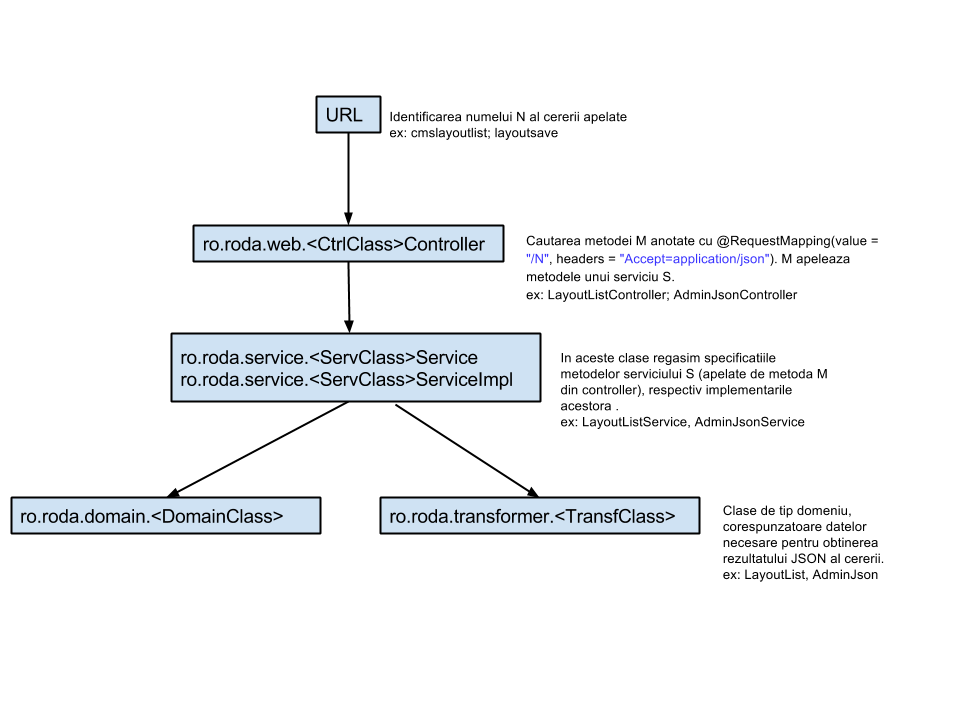
\includegraphics[width=\textwidth]{roda_URL.png}
\end{center}

\bigskip